\subsection{jExam UI-Tests}\label{subsec:jexam-ui-tests}

Diese Methode erm\"oglicht es, eine Plattform sowie ihre Funktionen anhand
ihrer grafischen Benutzeroberfl\"ache (\acs{ui} oder \gls{frontend}) zu
testen. Mit Hilfe moderner Werkzeuge und Frameworks ist es m\"oglich, die
Kontrolle \"uber einen Webbrowser vollautomatisch zu \"ubernehmen. Dies
erm\"oglicht es, das Verhalten eines Benutzers auf einer Weboberfl\"ache zu
simulieren. Es wurde bereits erw\"ahnt, dass \gls{jexam_2009} und \gls{jexam_new}
die gleiche grafische Benutzeroberfl\"ache haben. Es gibt jedoch einige
bemerkenswerte Unterschiede im Frontend-Code der beiden Plattformen,
die bei der Entwicklung von Tests Probleme verursachen k\"onnten
(siehe \Cref{fig:old_new}). Trotzdem gibt es eine
M\"oglichkeit, die Tests nur einmal und f\"ur alle zwei
Plattformen zu schreiben. Auf diese Weise sparen die Tester Zeit und k\"onnen
herausfinden, ob \gls{jexam_new} genauso gut funktioniert wie sein Vorg\"anger. Zu den Funktionen, die getestet werden müssen, gehören :
\begin{enumerate}
    \item Login
    \item Registrierung
    \item Abruf der Noten in der Übersicht
    \item Einschreibung in Prüfungen
    \item Einschreibung in Lehrveranstaltungen
    \item Einschreibung in Seminargruppen
\end{enumerate}

\noindent
\begin{figure}[H]
    \centering
    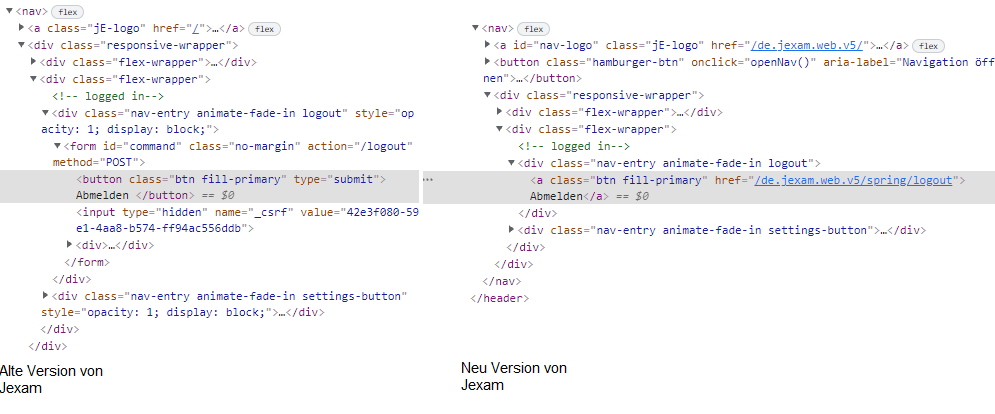
\includegraphics[scale=0.5]{images/jexam_compare}
    \caption{Frontend Quelltext von jExam 2009 und jExam new} \label{fig:old_new}
\end{figure}

